\documentclass[a4paper, 12pt]{article}
\usepackage{listings} 
\usepackage{xcolor}
\usepackage{mdframed}
\usepackage{graphicx}
\usepackage{pgfplots}
\usepackage{float}
\usepackage{mathtools}
\usepackage[margin=1.00in]{geometry}
\DeclarePairedDelimiter\ceil{\lceil}{\rceil}
\DeclarePairedDelimiter\floor{\lfloor}{\rfloor}
\definecolor{code-gray}{gray}{0.93}

% Beginning of Document
\begin{document}
% Title
\title{ECE 443 - Project \#5}
\author{Collin Heist}
\date{\today}
\maketitle

% Table of Content and Listings
\pagenumbering{roman}
\tableofcontents
\newpage
\pagenumbering{arabic}

% Beginning of Report
\section{Report}
Below, in \textbf{Figure~\ref{fig:can-buttons}}, a waveform capture of a typical transmission is shown. The CAN1 module initiates the communication (see the ID ending in 04), and CAN2 responds (ID 01) afterwards. This cycle is repeated every second.
	
\begin{figure}[H]
\centering
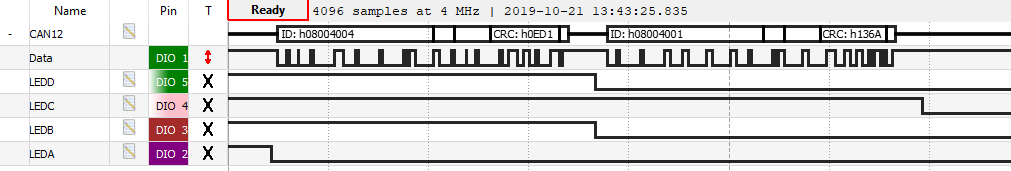
\includegraphics[width=\textwidth]{fig-can-buttons.PNG}
\caption{WaveForms capture of the CAN message and LED's}
\label{fig:can-buttons}
\end{figure}

The one-way communication timings are obtained by looking at how long it took between LEDA and LEDD toggling. LEDA is set when a transmission begins, and LEDD is set to the state of LEDA when it receives the message.  In my capture, I observed this as 323.5$\mu s$. 

\begin{figure}[H]
\centering
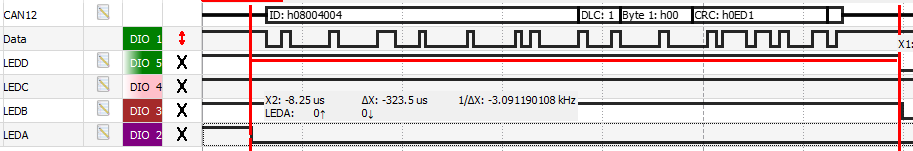
\includegraphics[width=\textwidth]{fig-one-way.PNG}
\caption{Timing of one-way communication over CAN}
\label{fig:one-way}
\end{figure}

Finally, I measured the timings for two-way communication. This was indicated by the toggle of LEDA, and terminated by the same toggle of LEDC (which indicates the 2nd message has been sent and received). This took 651.3$\mu s$, as shown in \textbf{Figure~\ref{fig:two-way}}. This is about what I expected, as a single transmission took almost exactly half this time.

\begin{figure}[H]
\centering
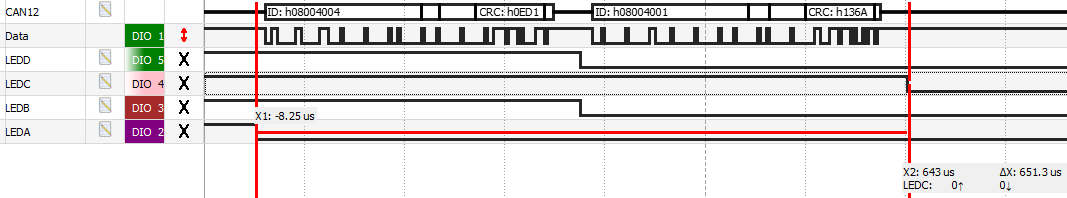
\includegraphics[width=\textwidth]{fig-two-way.PNG}
\caption{Timing of two-way communication over CAN}
\label{fig:two-way}
\end{figure}

\end{document}